\documentclass[a4paper, english]{report}

\usepackage[style=alphabetic]{biblatex}
\usepackage{blindtext}
\usepackage[utf8]{inputenc}
\usepackage{babel,csquotes,xpatch}
\usepackage{amsmath}
\usepackage{algorithm2e}
\usepackage{booktabs}
\usepackage{graphicx}


\DeclareMathOperator*{\argmax}{argmax}
\DeclareMathOperator*{\argmin}{argmin}
\DeclareMathOperator*{\simm}{sim}

\RestyleAlgo{algoruled}

\graphicspath{ {./images/} }

\addbibresource{bib/litRev.bib}

\begin{document}

\title{\Large{\textbf{Literature Review}}\\Batch Active Learning for Drug Discovery}
\author{rjb255}
\date{January 29, 2022}

\maketitle

\begin{abstract}
    \blindtext[1]{}
\end{abstract}

\section{Introduction}
\blindtext[2]{}

Scores displayed in examples have been based on the entire data set. Although this usually leads to data leakage within machine learning, this is not a concern here as the true comparison comes from testing  \textit{intelligent} vs \textit{dumb} learning methods. In both of these cases, the model is kept identical, but the selection process in not. The baseline simply takes the first $n$ entries from the data set, with the \textit{intelligent} method described where required. Three data sets have been used to demonstrate on multiple data sets [][][].

\section{Active Learning}\label{ch:Active Learning}
There are several schools of thought regarding active learning. These can be separated into two distinct categories: current data and future predictions. The former of these is computationally cheaper, as will be apparent on description.

\subsection{Current Data}
\subsubsection{Uncertainty Sampling}\label{sec:Uncertainty Sampling}
The simplest is applicable to cases in which a certainty is provided with each prediction. \textcite{LitRev_2009} suggests selecting the data point with the largest uncertainty according to the current model. Using the dataset '', this is demonstrated in [] with the algorithm for deciding the next sample point given in Alogrithm \ref{alg:US}.
\begin{algorithm}[H]
    \label{alg:US}
    \SetAlgoLined
    \KwData{$X_\mathrm{known}$, $Y_\mathrm{known}$, $X_\mathrm{unknown}$}
    \KwResult{Next $X$ to label}

    model = BayesianRidge()\;
    model.fit($X_\mathrm{known}$, $Y_\mathrm{known}$)\;
    standard\_deviation = model.standard\_deviation($X_\mathrm{unknown}$)\;
    \Return{max(standard\_deviation)}
    \caption{Uncertainty Sampling Selection}
\end{algorithm}

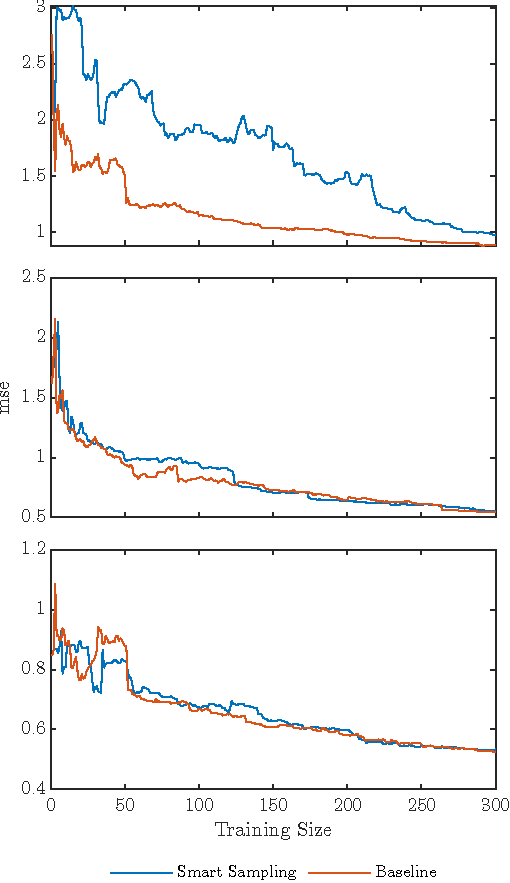
\includegraphics[width=100mm]{US_300_all3.pdf}

As addressed by \textcite{LitRev_2009}, this can be extended to any probabilistic model.
\begin{equation}
    \label{eq:x_next1}
    x_\mathrm{next}=\argmax_X{\left[s_{g(X)}\right]}
\end{equation}
\textcite{LitRev_2009} also notes the use of information theory for probabilistic models (\ref{eq:info_uncertainty}), where $y_i$ refers to all possible categorisations for $x$. This derives from the principle that the greatest entropy requires the most information to encode, and thus the least certain. However, \textcite{LitRev_2009} fails to address non-probabilistic models in this instance, instead converting such models into probabilistic ones.

\begin{equation}
    \label{eq:info_uncertainty}
    x_\mathrm{next}=\argmax_x{\left[-\sum_i{P(y_i|x)\ln{P(y_i|x)}}\right]}
\end{equation}

\subsubsection{Broad Knowledge Base}
A second form stems from information theory. Here, the aim is to produce an evenly dispersed $x$ allowing a well-informed knowledge base. There are two paths to proceed: density and nearest neighbours.

The former of these requires a definition of density in a sparsely populated space. As an analogy, the density of a gas appears well-defined, it becomes non-smooth once the volume defined over is comparable to the distance between particles. Thus, a new definition is required.

Alternatively, nearest neighbour requires little explanation. $x_\mathrm{next}$ is the unlabelled data point furthest from any labelled data point.

\begin{equation}
    \label{eq:inverseSim}
    x_\mathrm{next}=\argmax_x{\left(\sum{\frac{1}{\simm{(x, x_i)}}}\right)}
\end{equation}

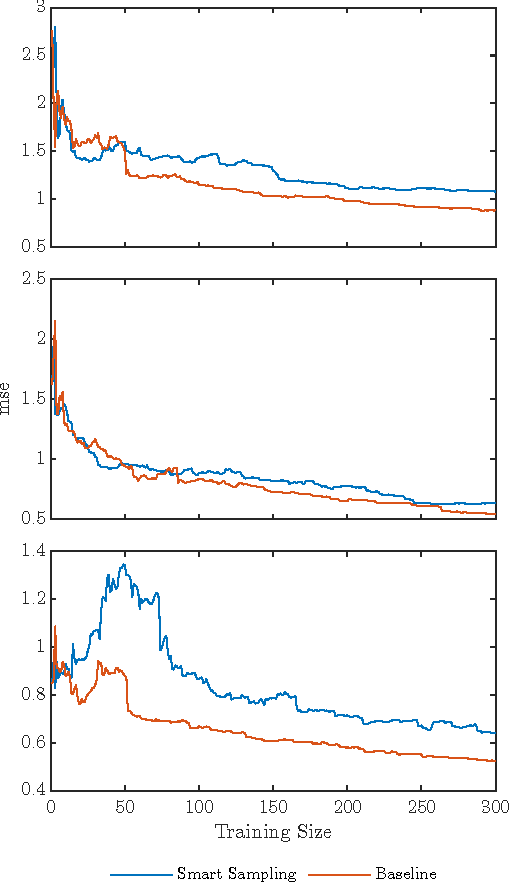
\includegraphics[width=100mm]{BKB_300_all3.pdf}

\subsubsection{Density Hotspots}
Conversely, a density weighted model has been suggested, as it escapes the introduction of error from outlier (i.e.\ data points far away from alternative data points). \textcite{Settles_2008} suggest (\ref{eq:Settles_density}) which can be broken down into two parts: a function for selection, $\phi_A$, and a function for similarity, $\simm$. The former arises from  another method described in this section. The latter requires a function to describe the similarity between data points.

\begin{equation}
    \label{eq:Settles_density}
    x_\mathrm{next}=\argmax_x{\left[\phi_A(x)\times{\left(\frac{1}{U}\sum{\simm{(x, x_i)}}\right)}^\beta\right]}
\end{equation}

\textcite{Settles_2008} admits that $\simm$ is open for interpretation. For simplicity, the average distance

\subsubsection{Regions of Disagreement}
As more complex methods are explored, we stumble across the method of competing hypothesis. This builds upon the [], and attempts to find []. The majority of work here relates to classification, although the same principles apply to regression. By minimising the region of disagreement between various models, a finer fit may be achieved.

One way of achieving this, especially in a regression model where boundaries are not quite so distinct, is to declare $n$ models ${M = \{m_1,\ldots{}, m_n\}}$. Combining these allow for a model $\hat{m}$ to be defined with prediction $\hat{y}$, being the mean prediction of $M$, ${\frac{1}{n}\sum{y_i}}$ and a sample standard deviation $\hat{s}$ defined as the sample standard deviation of $y_i$. This standard deviation can be used as a measure of the disagreement between the models. Thus, using a method as in Section~\ref{sec:Uncertainty Sampling}.

\subsection{Estimated Future}
These methods attempt to minimise a future attribute of the model. This works by predicting changes given with the inclusion of more data.

\subsubsection{Expected Model Change}

\section{Batch Active Learning}
Several naive methods are available here. Firstly, getting the top $N$ data points from a model described in Section~\ref{ch:Active Learning}. However, this method does not take into account the equivalence of the data points. This is extremely clear using the highest uncertainty method. It stands to reason that the area which has the highest uncertainty will see this for the data points nearest neighbours. Thus, this singular data point suffers the potential of being surrounded by $N-1$ other data points. The benefit this provides in fitting the model is thus extremely limited, and only slightly greater than if one data point had been chosen. A simple fix would be to simulate the model after 1 iteration, and select the next point from here. By doing this $N-1$ times, a better solution may be found, although this may prove to be computationally very expensive.
\subsection{Cluster-Margin}
\section{Drug Data}
\blindtext[2]{}

\printbibliography{}
\appendix

\end{document}